\section{Introduction}
\label{sec:intro}

Federated learning enables model training across distributed clients without sharing raw data, making it attractive for privacy-sensitive applications of LLMs \citep{kairouz2021advances}. Fine-tuning with LoRA \citep{hu2022lora} substantially reduces the number of trainable parameters per client, but federated LoRA aggregation still transmits nontrivial bytes per round. With 10 clients participating in every round across 15 rounds, the cumulative cost determines whether a protocol is deployable in bandwidth-constrained settings.

Existing federated LoRA methods differ in what they aggregate and when. FedIT \citep{zhang2024federatedgpt} applies FedAvg \citep{mcmahan2017communication} directly to LoRA's $A$ and $B$ matrices, paying full bidirectional cost per round. FFA-LoRA \citep{sun2024ffalora} freezes the $A$ matrix server-side and aggregates only $B$, achieving a theoretical 50\% upload savings once $A$ is frozen. FLoRA \citep{wang2024flora} stacks client LoRA modules and compresses via SVD, preserving product-space semantics at full bidirectional cost. FlexLoRA \citep{bai2024flexlora} supports heterogeneous client ranks and is orthogonal to the communication protocol studied here. All of these methods report communication savings as parameter-count ratios rather than measured bytes on the wire. None characterizes the asymmetric round that occurs when transitioning between aggregation modes. None uses an adaptive signal to select when to transition.

This paper addresses these gaps with three contributions.

\textbf{Bidirectional B-only protocol with measured byte tracking.}
The protocol implements both upload and download B-only transmission for Two-Phase and ReverseAdaptive aggregators. Per-round upload and download megabytes are recorded in experiment JSON files. The transition round, in which clients must upload full state to seed the server-side frozen $A$, is explicitly accounted for, producing a one-round asymmetry between when upload savings begin and when download savings begin.

\textbf{ReverseAdaptive: adaptive phase-switching aggregator.}
The aggregator starts in FLoRA mode and monitors the per-round loss improvement. When loss improvement falls below a threshold $\tau$ for the first time after a warmup period, the aggregator switches to FFA-LoRA permanently. By varying $\tau$, the adaptive aggregator recovers operating points equivalent to fixed-$K$ Two-Phase configurations without requiring $K$ to be selected in advance.

\textbf{Downstream evaluation and scale validation.}
This paper evaluates trained adapters on four zero-shot benchmarks MMLU \citep{hendrycks2020measuring}, ARC-Easy \citep{clark2018arc}, BoolQ \citep{clark2019boolq}, and HellaSwag \citep{zellers2019hellaswag} using log-likelihood scoring at two scales: TinyLlama-1.1B-Chat \citep{zhang2024tinyllama} for multi-seed IID and non-IID comparisons, and LLaMA-3.2-3B \citep{dubey2024llama3} with three-seed IID training and downstream evaluation.

\textbf{Headline numbers:}
Two-Phase $K{=}8$ saves 27.7\% (TinyLlama) and 26.0\% (LLaMA-3.2-3B) over FLoRA. ReverseAdaptive saves 40.5\% (TinyLlama) and $30.0 \pm 4.0$\% (LLaMA-3.2-3B, three seeds). At LLaMA-3.2-3B, ReverseAdaptive and Two-Phase $K{=}8$ produce statistically indistinguishable final losses (paired $t$-test, $p = 0.997$). All federated methods on LLaMA-3.2-3B cluster within 0.4 percentage points across all four downstream benchmarks.

Code, configuration files, and scripts to reproduce every figure and table are released in the public repository; see Appendix~\ref{app:repro}.

Section~\ref{sec:related} reviews related work. Section~\ref{sec:method} describes the protocol and ReverseAdaptive. Section~\ref{sec:experiments} presents experiments and results. Section~\ref{sec:discussion} provides discussion. Section~\ref{sec:limitations} lists limitations. Section~\ref{sec:conclusion} concludes.

\section{Related Work}
\label{sec:related}

\subsection{LoRA and Parameter-Efficient Fine-Tuning}
Parameter-efficient fine-tuning (PEFT) methods reduce the cost of adapting large pretrained models by training only a small subset of parameters. Adapter tuning \citep{houlsby2019parameter} inserts small trainable modules between transformer layers. LoRA \citep{hu2022lora} decomposes weight updates into low-rank products $BA$, where $B$ is $d \times r$ and $A$ is $r \times k$ with $r$ much smaller than $\min(d,k)$. This reduces trainable parameters substantially, enabling fine-tuning of large models without modifying base weights. QLoRA \citep{dettmers2023qlora} further reduces memory by quantizing the frozen base model to 4-bit while training LoRA adapters in 16-bit. The resulting LoRA adapters are compact and composable, making them a natural fit for federated settings where both storage and communication are constrained.

\subsection{Federated LoRA Aggregation}
FedIT \citep{zhang2024federatedgpt} applies standard FedAvg \citep{mcmahan2017communication} to LoRA matrices: the global $A$ and $B$ are computed as weighted averages of client $A$ and $B$ matrices. The aggregation introduces a mismatch: the optimal global update is the product $BA$, not a product of separately averaged $B$ and $A$. Averaging independently introduces aggregation error that grows with client heterogeneity.

FFA-LoRA \citep{sun2024ffalora} addresses the aggregation mismatch by freezing $A$ at initialization and training only $B$ across clients. Because $A$ is constant, the server aggregates $B$ matrices directly without product-space distortion. The theoretical upload saving is 50\%. The original work also motivates the frozen-$A$ design in terms of differential privacy. A critical difference from the protocol in this paper: FFA-LoRA freezes $A$ at initialization, whereas the bidirectional B-only protocol allows $A$ to be learned through a FLoRA phase before freezing, recovering expressivity at the cost of longer initial overhead.

FLoRA \citep{wang2024flora} preserves product-space semantics by stacking client LoRA modules horizontally and applying truncated SVD to recover a global low-rank adapter, reducing the aggregation bias present in FedIT. The tradeoff is communication cost: FLoRA transmits full $A{+}B$ payloads in both directions every round. FLoRA is the full-rank baseline in this paper's experiments.

FlexLoRA \citep{bai2024flexlora} extends federated LoRA to the heterogeneous-rank setting, where different clients use different LoRA ranks based on local compute budgets. FlexLoRA's contribution is orthogonal to this paper's; the bidirectional B-only protocol applies equally to homogeneous-rank clients.

\subsection{Communication-Efficient Federated Learning}
Communication efficiency in federated learning has been a central concern since FedAvg \citep{mcmahan2017communication} introduced local multi-step updates to reduce communication rounds. The broader challenge of open problems in federated learning is surveyed by \citet{kairouz2021advances}. Subsequent work has pursued per-round payload reduction through gradient compression. QSGD \citep{alistarh2017qsgd} reduces the bit-width of transmitted gradients through stochastic quantization. Deep gradient compression \citep{lin2017deep} applies aggressive sparsification, sending only 0.1\% of gradients per round with error feedback. FedPAQ \citep{reisizadeh2020fedpaq} combines periodic averaging with quantization, showing that 8-bit transmission incurs negligible accuracy loss. These techniques are orthogonal to the B-only protocol studied here and could in principle be composed with it for additional savings.

\subsection{Adaptive Aggregation and Scheduling}
Several federated learning methods adapt their behavior based on observed training dynamics. FedProx \citep{li2020fedprox} adds an adaptive proximal term to the local objective, controlling deviation from the global model. FedNova \citep{wang2020fednova} normalizes local gradients by effective step count, adaptively correcting for heterogeneous local training. FedAdam and FedYogi \citep{reddi2020adaptive} apply adaptive moment estimation at the server level, treating the aggregated pseudo-gradient as input to Adam-style updates. Curriculum scheduling in federated learning adjusts the aggregation frequency over training, structurally related to ReverseAdaptive's phase-switching in that both methods behave differently early vs.\ late in training. To the authors' knowledge, no prior federated LoRA work uses a loss-plateau signal to switch between distinct aggregation modes during training.

\section{Method}
\label{sec:method}

\subsection{Background and Notation}
Each of $N$ clients holds a local dataset. A shared base model has weight matrices $W$. LoRA \citep{hu2022lora} parameterizes updates as $\Delta W = BA$ where $B$ is $d \times r$ and $A$ is $r \times k$. In each federated round, clients train their local adapters for one epoch, upload some representation to the server, and receive a global state.

The communication cost of a round is the sum of upload bytes and download bytes. For TinyLlama-1.1B with rank $r{=}16$ targeting $\{\texttt{q\_proj}, \texttt{k\_proj}, \texttt{v\_proj}, \texttt{o\_proj}\}$ layers, accounting for GQA in the key/value projections, the B-only fraction of the full state is approximately 36\% rather than the 50\% a naive parameter count would suggest. LLaMA-3.2-3B has a B-only fraction of approximately 40\% due to different GQA configuration.

\subsection{Bidirectional B-Only Protocol}
\textbf{Phase 1 (FLoRA, rounds 1 to $K$).}
The server runs FLoRA aggregation \citep{wang2024flora}: client states are stacked and compressed via SVD to produce a global $(A_{\text{global}}, B_{\text{global}})$. Both upload and download payloads are full state.

\textbf{Transition (round $K{+}1$).}
Clients still upload full state $(A_i, B_i)$ because the server needs the $A$ matrices to compute and cache $A_{\text{frozen}}$. The server runs FFA-LoRA \citep{sun2024ffalora} aggregation for the first time, caches $A_{\text{frozen}}$, and broadcasts the full global state.

\textbf{Phase 2 steady state (rounds $K{+}2$ onward).}
Clients upload only $B_i$; the server reconstructs the full state as $(A_{\text{frozen}}, B_i)$ before aggregation. The server broadcasts only $B_{\text{global}}$; clients retain $A_{\text{frozen}}$ locally.

\textbf{Look-ahead download accounting.}
This produces a one-round asymmetry: download savings begin one round before upload savings. The experiment runner records this consistently, ensuring reported totals are accurate rather than optimistic.

Algorithm~\ref{alg:bonly} specifies the server-side decision logic per round.

\begin{algorithm}[t]
\caption{Bidirectional B-only protocol (server, per round)}
\label{alg:bonly}
\begin{algorithmic}[1]
\Require round $r$, phase boundary $K$, frozen-$A$ cache (initially empty)
\Ensure upload mode, broadcast mode
\If{$r \leq K$} \Comment{FLoRA phase}
    \State upload $\leftarrow$ full state $(A, B)$
    \State broadcast $\leftarrow$ full state
\ElsIf{$r = K+1$} \Comment{transition: seeds $A_{\text{frozen}}$}
    \State upload $\leftarrow$ full state
    \State $A_{\text{frozen}} \leftarrow$ cache server $A$ matrices
    \State broadcast $\leftarrow$ full state
\Else \Comment{FFA-LoRA steady state}
    \State upload $\leftarrow$ $B$ only \Comment{server prepends $A_{\text{frozen}}$}
    \State broadcast $\leftarrow$ $B$ only \Comment{clients retain $A_{\text{frozen}}$ locally}
\EndIf
\end{algorithmic}
\end{algorithm}

\subsection{ReverseAdaptive Aggregator}
ReverseAdaptive replaces the fixed boundary $K$ with an adaptive loss-plateau signal. After a warmup period of $W$ rounds (default $W{=}5$), it monitors the per-round loss improvement $\Delta\ell_r = \ell_{r-1} - \ell_r$. When $\Delta\ell_r < \tau$ for the first time, the aggregator switches to FFA-LoRA \citep{sun2024ffalora} mode permanently. A complementary stability detector reverts to FLoRA if loss increases by more than 10\% after switching; no reverts occurred across all 21 ReverseAdaptive runs in this study (3 IID seeds + 3 Non-IID $\alpha{=}0.5$ + 5 Non-IID $\alpha{=}0.1$ + 8 threshold-ablation + 3 LLaMA-3.2-3B IID + 1 no-switch sanity).

The choice of $\tau$ trades communication savings against final training loss. Small $\tau$ delays the switch; large $\tau$ triggers it at the first eligible round after warmup. Section~\ref{sec:ablation} characterizes this tradeoff empirically.

The choice of loss-plateau as the switching signal reflects an empirical observation about federated LoRA training dynamics. In the early phase of training, the $A$ matrices carry meaningful task-specific gradient information, and full-rank aggregation contributes to convergence. As training progresses and the loss landscape begins to flatten, $A$ approaches a stable configuration; the additional expressivity gained from continuing to aggregate it is marginal. At this point, FFA-LoRA's frozen-$A$ approximation becomes a near-lossless substitute for full-rank aggregation. Plateau detection is therefore a natural proxy for the condition that $A$ has converged enough to be frozen safely. Alternative signals such as gradient norm of $A$ or the singular value spectrum of stacked client matrices could in principle provide more direct measures, but the loss-plateau signal is chosen here for its simplicity, its availability without additional instrumentation, and the fact that it tracks the quantity the practitioner cares about most directly.

Algorithm~\ref{alg:reverseadaptive} specifies the aggregator's per-round decision logic.

\begin{algorithm}[t]
\caption{ReverseAdaptive aggregator (per round)}
\label{alg:reverseadaptive}
\begin{algorithmic}[1]
\Require round $r$, current loss $\ell_r$, prior loss $\ell_{r-1}$,
         warmup $W$, threshold $\tau$, current mode $m$, \texttt{client\_states}
\Ensure \texttt{global\_state}, updated mode $m$
\If{$m = \text{FLoRA}$ \textbf{and} $r > W$ \textbf{and} $(\ell_{r-1} - \ell_r) < \tau$}
    \State $m \leftarrow \text{FFA-LoRA}$
    \State log event $(r, \texttt{switch\_to\_ffa})$
\ElsIf{$m = \text{FFA-LoRA}$ \textbf{and} $\ell_r > 1.1 \cdot \ell_{r-1}$} \Comment{stability revert}
    \State $m \leftarrow \text{FLoRA}$
    \State reset $A_{\text{frozen}}$
    \State log event $(r, \texttt{revert\_to\_flora})$
\EndIf
\If{$m = \text{FFA-LoRA}$}
    \State \Return \textsc{FFA-LoRA-Aggregate}(\texttt{client\_states})
\Else
    \State \Return \textsc{FLoRA-Aggregate}(\texttt{client\_states})
\EndIf
\end{algorithmic}
\end{algorithm}

\subsection{Implementation Details}
\textbf{Byte tracking.}
Per-round upload and download megabytes are recorded in \texttt{results.json}. Byte counts use bfloat16 (2 bytes/param) for TinyLlama, float16 base with float32 LoRA for LLaMA-3.2-3B. All models are optimized using AdamW \citep{loshchilov2019decoupled}.

\textbf{GQA B-fraction.}
TinyLlama-1.1B's GQA makes the B-only fraction approximately 36\%, not 50\%. LLaMA-3.2-3B's B-only fraction is approximately 40\%. These architectural differences affect absolute savings numbers across scales and are reported explicitly.

\textbf{Partition mechanics.}
Non-IID partitions use Dirichlet label-skew with $\alpha \in \{0.5, 0.1\}$. Under severe skew ($\alpha{=}0.1$), some clients may receive empty partitions; per-seed active client counts are in Appendix~\ref{app:perseed}.

\section{Experiments and Results}
\label{sec:experiments}

\subsection{Setup}
Table~\ref{tab:setup} summarizes the experimental configuration. Total compute was approximately 285 hours on Apple M4 Pro hardware; no external GPU was used. Both TinyLlama-1.1B and LLaMA-3.2-3B experiments use three seeds for IID training.

\begin{table}[t]
\caption{Experimental setup.}
\label{tab:setup}
\begin{center}
\begin{tabular}{ll}
\toprule
Parameter & Value \\
\midrule
Base models & TinyLlama-1.1B-Chat-v1.0 \citep{zhang2024tinyllama}; \\
            & LLaMA-3.2-3B \citep{dubey2024llama3} \\
Dataset & Alpaca \citep{taori2023alpaca}, 3000 samples \\
Data partitions & IID; Dirichlet $\alpha{=}0.5$; Dirichlet $\alpha{=}0.1$ \\
Clients / round & 10 / 10 (full participation) \\
Rounds & 15 \\
Local epochs & 1 \\
Batch size & 4 (TinyLlama), 2 (LLaMA-3.2-3B) \\
Grad.\ accumulation & 4 (TinyLlama), 8 (LLaMA-3.2-3B); effective batch 16 \\
Learning rate & $10^{-4}$ (AdamW; \citealt{loshchilov2019decoupled}) \\
Max sequence length & 256 \\
LoRA rank / alpha & 16 / 32 \\
LoRA target modules & \texttt{q\_proj}, \texttt{k\_proj}, \texttt{v\_proj}, \texttt{o\_proj} \\
LoRA dropout & 0.1 \\
Hardware & Apple M4 Pro, 48\,GB unified memory, MPS \\
Model dtype & bfloat16 (TinyLlama); float16 base + float32 LoRA (LLaMA) \\
Downstream eval & 500 examples/benchmark, seed 42, log-likelihood \\
Benchmarks & MMLU \citep{hendrycks2020measuring}, ARC-Easy \citep{clark2018arc}, \\
            & BoolQ \citep{clark2019boolq}, HellaSwag \citep{zellers2019hellaswag} \\
Seeds (TinyLlama IID) & \{42, 123, 456\} \\
Seeds (LLaMA-3.2-3B) & \{42, 123, 456\} \\
ReverseAdaptive defaults & \texttt{warmup\_rounds}=5, $\tau{=}0.01$, \texttt{stability\_threshold}=1.1 \\
\bottomrule
\end{tabular}
\end{center}
\end{table}

\subsection{Communication-Quality Pareto Curve}
Table~\ref{tab:tinyllama_iid} and Figure~\ref{fig:pareto} show the communication-quality tradeoffs on TinyLlama-1.1B \citep{zhang2024tinyllama} under IID partitioning. FLoRA \citep{wang2024flora} establishes the baseline at 2578 MB total communication and final loss 1.2605. Two-Phase $K{=}10$ reduces communication to 2083 MB (19.2\% savings) with final loss 1.2665. Two-Phase $K{=}8$ reduces further to 1863 MB (27.7\% savings) with final loss 1.2703. ReverseAdaptive at $\tau{=}0.01$ achieves 1533 MB (40.5\% savings) with final loss 1.2746.

\begin{figure}[ht]
\begin{center}
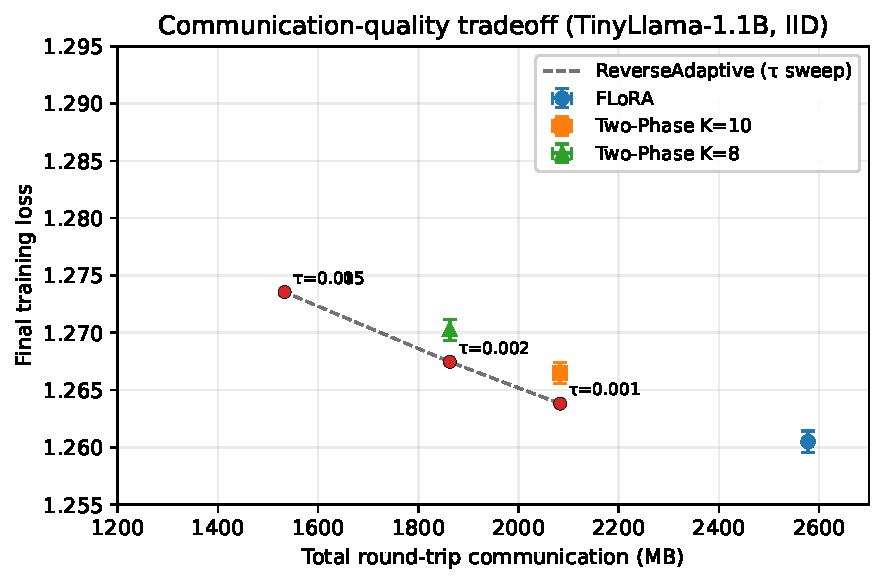
\includegraphics[width=0.85\linewidth]{figures/fig1_pareto_iid.pdf}
\end{center}
\caption{Communication-quality Pareto curve on Alpaca-3k, TinyLlama-1.1B, IID.
Fixed-$K$ Two-Phase points (mean $\pm$ 1 standard deviation over three seeds) lie
on a curve traced by ReverseAdaptive's threshold parameter $\tau$. The dashed
connector shows $\tau \in \{0.001, 0.002, 0.005, 0.01\}$. FLoRA is the no-savings
baseline at upper right; ReverseAdaptive at $\tau \geq 0.005$ is the maximum-savings
configuration at lower left.}
\label{fig:pareto}
\end{figure}

The ReverseAdaptive points trace a Pareto frontier from (1533 MB, 1.274) at $\tau \geq 0.005$ to (2083 MB, 1.264) at $\tau{=}0.001$. This frontier sweeps through the fixed-$K$ Two-Phase operating points: $\tau{=}0.002$ reproduces Two-Phase $K{=}8$ communication exactly, and $\tau{=}0.001$ reproduces $K{=}10$. The adaptive method recovers the full fixed-$K$ Pareto frontier without requiring $K$ to be specified.

Loss differences between methods are small in absolute terms (0.014 between FLoRA and ReverseAdaptive at $\tau{=}0.01$) but statistically distinguishable across three seeds (paired $t$-tests, $p < 10^{-4}$). Full statistical tests are in Appendix~\ref{app:stats}.

\begin{table}[t]
\caption{TinyLlama-1.1B IID results (3 seeds, mean $\pm$ std).
Communication is deterministic across seeds.}
\label{tab:tinyllama_iid}
\begin{center}
\begin{tabular}{lcccc}
\toprule
Method & Final loss & Total comm.\ (MB) & Savings vs.\ FLoRA & $p$-value \\
\midrule
FLoRA \citep{wang2024flora}            & $1.2605 \pm 0.0009$ & 2578.13 & -- & -- \\
Two-Phase $K{=}10$                     & $1.2665 \pm 0.0009$ & 2083.13 & 19.20\% & $2.5 \times 10^{-5}$ \\
Two-Phase $K{=}8$                      & $1.2703 \pm 0.0009$ & 1863.13 & 27.73\% & $2.5 \times 10^{-5}$ \\
ReverseAdaptive ($\tau{=}0.01$)        & $1.2746 \pm 0.0009$ & 1533.13 & 40.53\% & $6.1 \times 10^{-6}$ \\
\bottomrule
\end{tabular}
\end{center}
\end{table}

\subsection{Convergence and Switching Behavior}
Figure~\ref{fig:convergence} shows mean $\pm$ std loss trajectories across three seeds for FLoRA, Two-Phase $K{=}8$, and ReverseAdaptive. All three methods converge similarly through the FLoRA phase. Phase transitions are visible as slight slope changes but do not destabilize training. The final ${\sim}0.01$ loss gap accumulates gradually after the switch rather than appearing as a sharp discontinuity.

\begin{figure}[t]
\begin{center}
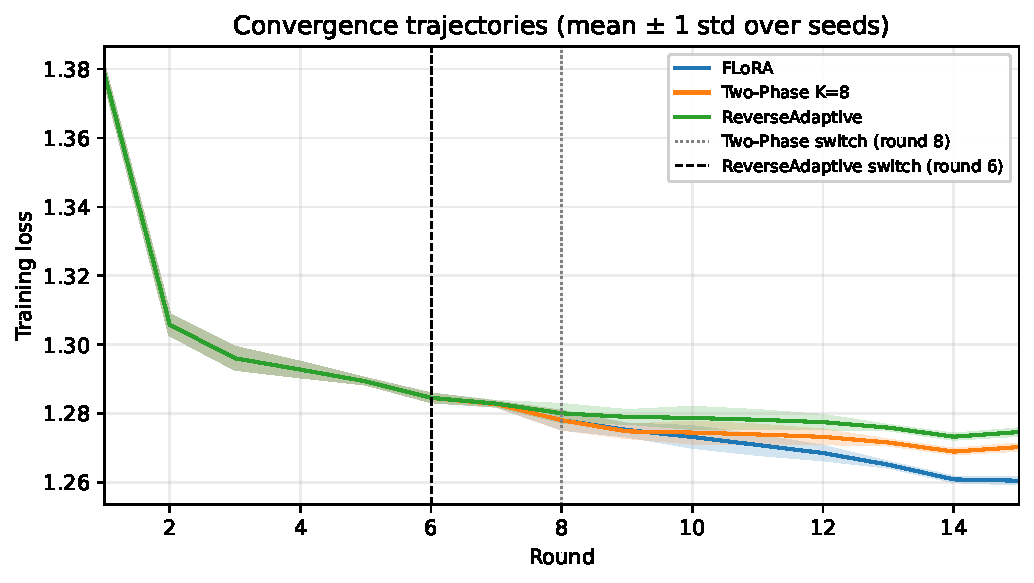
\includegraphics[width=0.85\linewidth]{figures/fig2_convergence.pdf}
\end{center}
\caption{Training loss trajectories on TinyLlama-1.1B IID. Mean $\pm$ 1 standard deviation over three seeds. Vertical dashed lines mark ReverseAdaptive's switch round (round 6) and Two-Phase $K{=}8$'s phase boundary (round 8). All three methods converge similarly through the FLoRA phase; the loss gap accumulates gradually after the switch.}
\label{fig:convergence}
\end{figure}

Figure~\ref{fig:cumcomm} shows cumulative communication in megabytes against round number for TinyLlama-1.1B. FLoRA stays linear at 85.94 MB per round per direction throughout. Two-Phase $K{=}8$ maintains the same slope through round 9, then reduces as B-only transmission activates. ReverseAdaptive splits off at round 6 (at TinyLlama-1.1B scale), producing the steepest savings trajectory.

\begin{figure}[t]
\begin{center}
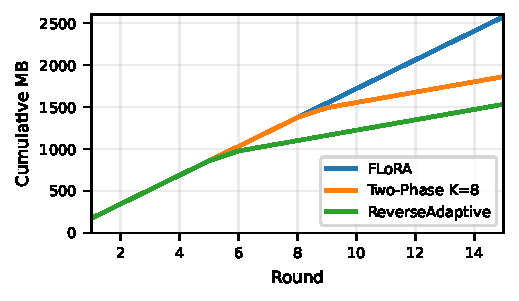
\includegraphics[width=0.85\linewidth]{figures/fig3_cumulative_comm.pdf}
\end{center}
\caption{Cumulative communication on TinyLlama-1.1B (seed 42, deterministic across seeds). Slope changes mark phase transitions: ReverseAdaptive at round 6, Two-Phase $K{=}8$ at round 9. The look-ahead download accounting causes the broadcast slope to change one round before the upload slope changes.}
\label{fig:cumcomm}
\end{figure}

The no-switch sanity baseline (ReverseAdaptive with \texttt{switch\_threshold} $= -1.0$, \texttt{warmup\_rounds} $= 999$) produces final loss 1.2594342812 on seed 42, matching the FLoRA seed 42 result to 10 decimal places. Upload and download match to the byte across all 15 rounds.

\subsection{Downstream Evaluation}
Tables~\ref{tab:downstream_tiny}--\ref{tab:downstream_llama} and Figure~\ref{fig:downstream} present downstream results on MMLU \citep{hendrycks2020measuring}, ARC-Easy \citep{clark2018arc}, BoolQ \citep{clark2019boolq}, and HellaSwag \citep{zellers2019hellaswag}. MMLU is excluded from TinyLlama-1.1B comparisons: base accuracy of 0.250 on 4-way multiple choice indicates chance-level performance, making the benchmark uninformative at 1.1B scale.

\begin{figure}[t]
\begin{center}
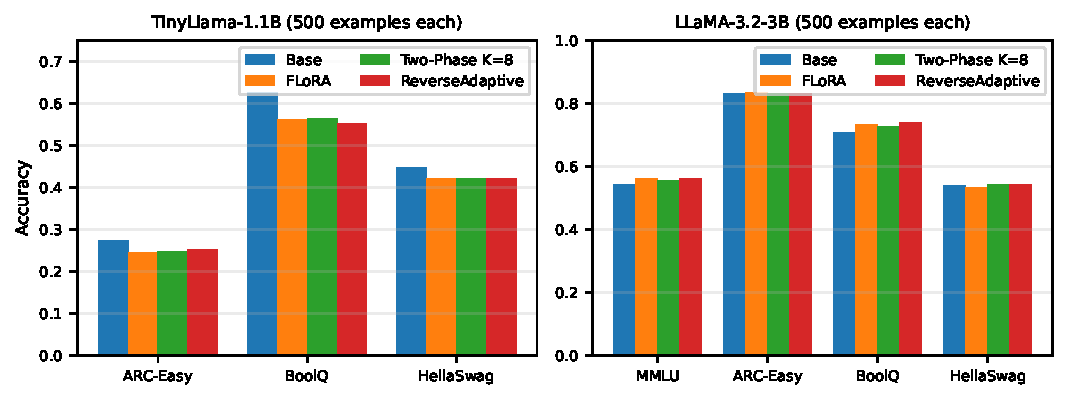
\includegraphics[width=0.85\linewidth]{figures/fig4_downstream_accuracy.pdf}
\end{center}
\caption{Downstream zero-shot accuracy across two model scales (500 examples per benchmark). Left: TinyLlama-1.1B (seed 42 only; ARC-Easy, BoolQ, HellaSwag; MMLU omitted because base accuracy is at chance for 4-way multiple choice). Right: LLaMA-3.2-3B (mean across three seeds; MMLU, ARC-Easy, BoolQ, HellaSwag). Federated methods cluster within 1.4 percentage points at TinyLlama-1.1B and 0.4 percentage points at LLaMA-3.2-3B.}
\label{fig:downstream}
\end{figure}

At TinyLlama-1.1B (Table~\ref{tab:downstream_tiny}), all federated methods cluster within 1.4 percentage points of each other. All methods regress modestly relative to the base model. The base model's BoolQ accuracy of 0.626 closely matches BoolQ's natural yes-class rate of approximately 0.62, suggesting the base exploits a yes-biased prior. Federated Alpaca-3k instruction tuning attenuates this prior, producing regression across all methods uniformly.

At LLaMA-3.2-3B scale, the three federated methods are statistically indistinguishable on downstream benchmarks. Mean accuracies across three seeds differ by at most 0.4 percentage points on any benchmark, and all cross-method differences lie within the seed-to-seed standard deviation of each individual method. The picture differs from the TinyLlama panel in two ways. The federated methods are flat to slightly positive relative to the base model at 3B rather than regressing as they did at 1.1B; the LLaMA base achieves MMLU 0.544, ARC-Easy 0.832, BoolQ 0.706, and HellaSwag 0.540, and federated methods either match or slightly exceed each of these. The within-method seed variance is also smaller at 3B than the within-scale spread observed at TinyLlama, indicating that downstream benchmarks become more stable as model capacity grows.

\begin{table}[t]
\caption{Downstream zero-shot accuracy, TinyLlama-1.1B. MMLU omitted: base accuracy is at chance for 4-way multiple choice.}
\label{tab:downstream_tiny}
\begin{center}
\begin{tabular}{lcccc}
\toprule
Method & ARC-Easy & BoolQ & HellaSwag & $\Delta$ vs.\ base (BoolQ) \\
\midrule
Base (no adapter) & 0.274 & 0.626 & 0.448 & -- \\
FLoRA             & 0.246 & 0.562 & 0.420 & $-6.4$ pp \\
Two-Phase $K{=}8$ & 0.248 & 0.560 & 0.420 & $-6.6$ pp \\
ReverseAdaptive   & 0.252 & 0.552 & 0.420 & $-7.4$ pp \\
Spread (max--min) & 0.006 & 0.010 & 0.000 & -- \\
\bottomrule
\end{tabular}
\end{center}
\end{table}

\begin{table}[t]
\caption{Downstream zero-shot accuracy, LLaMA-3.2-3B. Mean $\pm$ 1 standard deviation across three random seeds (42, 123, 456). 500 examples per benchmark. Cross-method spread is at most 0.4 percentage points on any benchmark and is within the seed-to-seed standard deviation of each method.}
\label{tab:downstream_llama}
\begin{center}
\begin{tabular}{lcccc}
\toprule
Method & MMLU & ARC-Easy & BoolQ & HellaSwag \\
\midrule
Base (no adapter) & 0.544 & 0.832 & 0.706 & 0.540 \\
FLoRA             & $0.558 \pm 0.007$ & $0.836 \pm 0.007$ & $0.736 \pm 0.007$ & $0.535 \pm 0.003$ \\
Two-Phase $K{=}8$ & $0.558 \pm 0.002$ & $0.837 \pm 0.008$ & $0.738 \pm 0.010$ & $0.539 \pm 0.004$ \\
ReverseAdaptive   & $0.557 \pm 0.003$ & $0.839 \pm 0.008$ & $0.739 \pm 0.004$ & $0.538 \pm 0.004$ \\
\bottomrule
\end{tabular}
\end{center}
\end{table}

\subsection{Threshold Ablation}
\label{sec:ablation}
Table~\ref{tab:ablation} and Figure~\ref{fig:ablation} characterize how $\tau$ controls the savings-quality tradeoff. The method has a sensitive regime for $\tau \leq 0.002$: at $\tau{=}0.002$ the switch occurs at round 9, matching Two-Phase $K{=}8$; at $\tau{=}0.001$ the switch occurs at round 11, matching Two-Phase $K{=}10$. For $\tau \geq 0.005$ the method saturates: the switch fires at round 6, the first round after warmup. All rows for $\tau \in \{0.005, 0.010, 0.020, 0.050, 0.100, 0.200\}$ produce identical results.

\begin{figure}[t]
\begin{center}
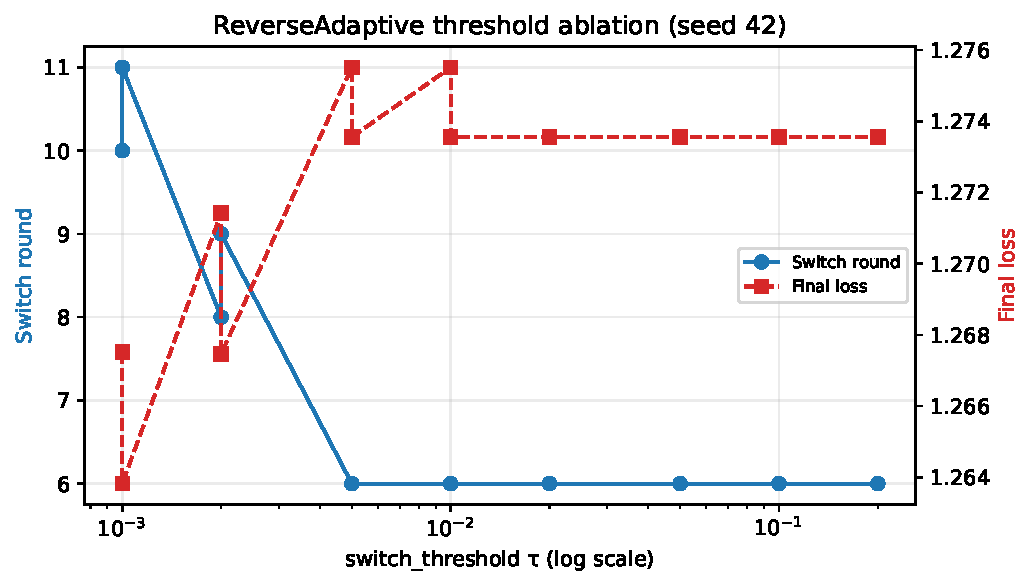
\includegraphics[width=0.85\linewidth]{figures/fig5_threshold_ablation.pdf}
\end{center}
\caption{ReverseAdaptive threshold sensitivity (TinyLlama-1.1B IID, seed 42). Switch round (left axis, blue) and final training loss (right axis, red) plotted against $\tau$ on logarithmic scale. Sensitive regime for $\tau \leq 0.002$; saturation at first eligible round for $\tau \geq 0.005$.}
\label{fig:ablation}
\end{figure}

A practitioner seeking maximum savings can set $\tau$ anywhere in $[0.005, 0.2]$ without precision loss. The $\tau{=}0.001$ and $\tau{=}0.002$ operating points demonstrate that the adaptive method genuinely tracks the loss trajectory rather than saturating trivially.

\begin{table}[t]
\caption{ReverseAdaptive threshold sensitivity (TinyLlama IID, seed 42).}
\label{tab:ablation}
\begin{center}
\begin{tabular}{lcccc}
\toprule
$\tau$ & Switch round & Final loss & Total comm.\ (MB) & Savings \\
\midrule
0.001 & 11 & 1.2638 & 2083.13 & 19.20\% \\
0.002 & 9  & 1.2675 & 1863.13 & 27.73\% \\
0.005 & 6  & 1.2736 & 1533.13 & 40.53\% \\
0.010 & 6  & 1.2736 & 1533.13 & 40.53\% \\
0.020 & 6  & 1.2736 & 1533.13 & 40.53\% \\
0.050 & 6  & 1.2736 & 1533.13 & 40.53\% \\
0.100 & 6  & 1.2736 & 1533.13 & 40.53\% \\
0.200 & 6  & 1.2736 & 1533.13 & 40.53\% \\
\bottomrule
\end{tabular}
\end{center}
\end{table}

\subsection{Scale Validation}
Table~\ref{tab:llama_iid} and Figure~\ref{fig:scale} confirm that the Pareto structure observed at TinyLlama-1.1B is preserved at LLaMA-3.2-3B. Three random seeds (42, 123, 456) were run for each of FLoRA, Two-Phase $K{=}8$, and ReverseAdaptive, producing nine total runs. Final-round results (mean $\pm$ standard deviation): FLoRA reaches loss $1.3724 \pm 0.0009$ with 2625.0 MB total communication. Two-Phase $K{=}8$ reaches loss $1.3938 \pm 0.0011$ with 1942.5 MB (savings 26.0\%). ReverseAdaptive reaches loss $1.3938 \pm 0.0036$ with $1837.5 \pm 105.0$ MB (savings $30.0 \pm 4.0$\%). The protocol-deterministic communication for FLoRA and Two-Phase $K{=}8$ produces zero seed-to-seed variance; ReverseAdaptive's variance reflects across-seed differences in switch round (7, 8, 9 across the three seeds, mean $8.0 \pm 1.0$).

\begin{figure}[t]
\begin{center}
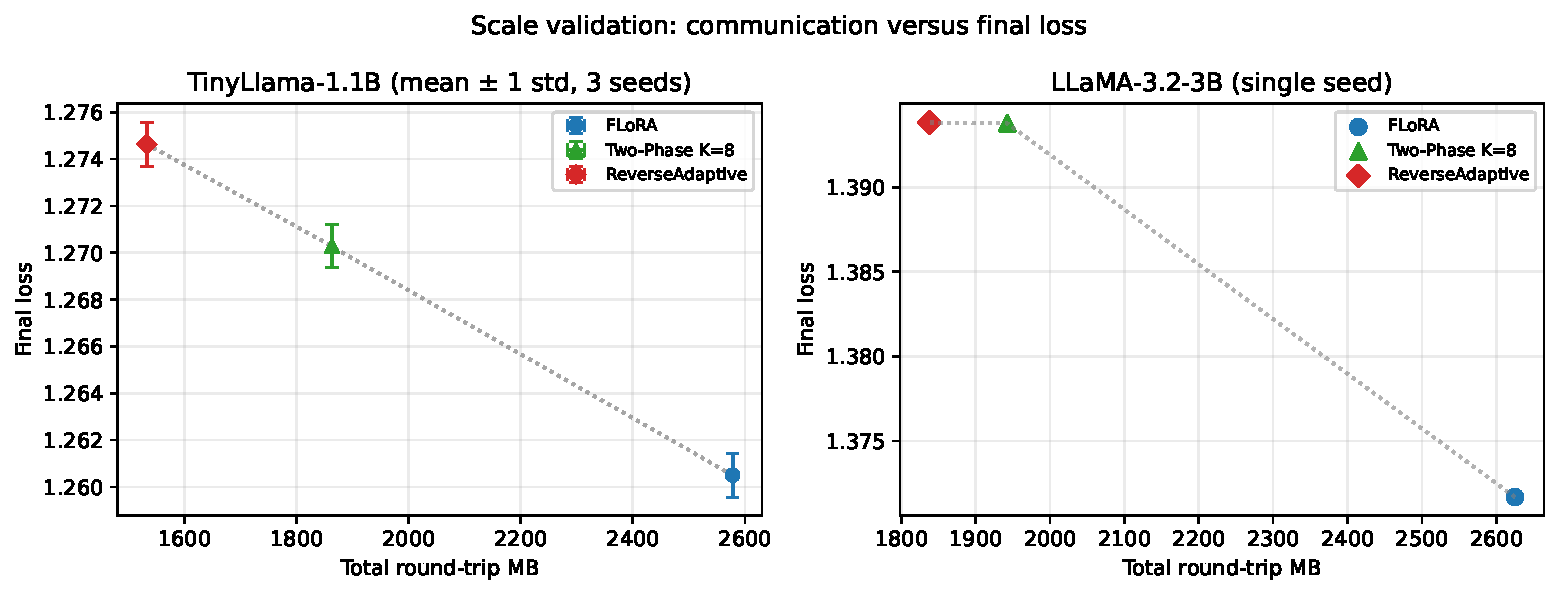
\includegraphics[width=0.85\linewidth]{figures/fig6_scale_validation.pdf}
\end{center}
\caption{Scale validation. Left: TinyLlama-1.1B (mean $\pm$ 1 standard deviation over three seeds). Right: LLaMA-3.2-3B (mean $\pm$ 1 standard deviation over three seeds). Both panels show the three federated methods on the same axes. Dotted polyline connects the three method points on each panel. The Pareto structure (downward slope from FLoRA to ReverseAdaptive) is preserved across scales. Y-axis ranges differ between panels because absolute training loss is model-dependent; the relative Pareto shape is the invariant being validated. ReverseAdaptive's larger error bar at LLaMA-3.2-3B reflects across-seed variance in switch round (7, 8, 9).}
\label{fig:scale}
\end{figure}

The communication savings are slightly lower at 3B than at 1.1B: 26.0\% vs.\ 27.7\% for Two-Phase $K{=}8$, and 30.0\% vs.\ 40.5\% for ReverseAdaptive. The B-only fraction of the full state is 40\% at LLaMA-3.2-3B (vs.\ 36\% for TinyLlama) due to different GQA configurations, meaning each B-only round saves a smaller fraction of the full payload at 3B scale.

ReverseAdaptive and Two-Phase $K{=}8$ produce statistically indistinguishable final losses at LLaMA-3.2-3B scale (paired $t$-test across three seeds: $p = 0.997$, Cohen's $d = 0.003$). The adaptive method achieves the same operating point that hand-tuned Two-Phase $K{=}8$ reaches, while saving an additional 4.0 percentage points of mean communication (30.0\% vs.\ 26.0\%) by occasionally switching at round 7 instead of round 8 or 9. Notably, ReverseAdaptive arrived at this operating point with no scale-specific hyperparameter tuning; the same threshold $\tau{=}0.01$ used at TinyLlama-1.1B produces a switch round that matches the hand-tuned $K{=}8$ configuration on average at LLaMA-3.2-3B.

\begin{table}[t]
\caption{LLaMA-3.2-3B IID results. Mean $\pm$ 1 standard deviation across three random seeds (42, 123, 456). ReverseAdaptive switch rounds: 7, 8, 9. FLoRA and Two-Phase $K{=}8$ communication is protocol-deterministic; ReverseAdaptive communication varies with switch round.}
\label{tab:llama_iid}
\begin{center}
\begin{tabular}{lccc}
\toprule
Method & Final loss & Total MB & Savings vs.\ FLoRA \\
\midrule
FLoRA & $1.3724 \pm 0.0009$ & 2625.0 & 0\% \\
Two-Phase $K{=}8$ & $1.3938 \pm 0.0011$ & 1942.5 & 26.0\% \\
ReverseAdaptive ($\tau{=}0.01$) & $1.3938 \pm 0.0036$ & $1837.5 \pm 105.0$ & $30.0 \pm 4.0$\% \\
\bottomrule
\end{tabular}
\end{center}
\end{table}

\section{Discussion}
\label{sec:discussion}

\subsection{Implications for Federated LLM Deployment}
The 40.5\% communication savings ReverseAdaptive achieves on TinyLlama-1.1B, and 30.0\% on LLaMA-3.2-3B, translate directly into reduced network costs in real deployments. In mobile or IoT federated settings where uplink bandwidth is scarce and metered, a protocol that cuts round-trip communication by 30--40\% without downstream quality loss can change the economic viability of federated fine-tuning entirely. Prior work by \citet{kairouz2021advances} identifies communication as one of the fundamental open problems in federated learning at scale. The byte-tracking framework and adaptive protocol introduced in this paper are a concrete step toward addressing that problem in the specific context of LLM fine-tuning.

\subsection{Why Adaptive Outperforms Fixed-$K$}
The Two-Phase protocol requires a practitioner to select $K$ before training begins, without knowing when the loss plateau will occur for a given model-dataset combination. This is a hyperparameter that must be tuned per dataset, per model, and potentially per client population: precisely the kind of manual configuration that slows deployment in production federated systems. ReverseAdaptive eliminates this by monitoring the signal that $K$ was meant to approximate.

The cross-scale result validates that the plateau signal is tracking genuine training dynamics rather than an arbitrary threshold. Using the same $\tau{=}0.01$ at TinyLlama-1.1B and LLaMA-3.2-3B, ReverseAdaptive fires at round 6 and at a mean of round $8.0 \pm 1.0$ respectively, automatically aligning with what a hand-tuned $K{=}8$ would select at 3B scale. No scale-specific retuning was required. This zero-cost scale transfer is the most practically significant finding in this paper: it suggests that $\tau$ may be stable across a range of model sizes and tasks, making ReverseAdaptive a drop-in replacement for Two-Phase in production pipelines.

The within-scale variance of switch rounds at LLaMA-3.2-3B (7, 8, 9 across three seeds) provides additional evidence that the adaptive method is responding to actual training dynamics rather than firing at the warmup boundary. Different random initializations produce slightly different loss trajectories, and ReverseAdaptive correctly responds to each. The mean switch round of $8.0 \pm 1.0$ matches the hand-tuned $K{=}8$ configuration on average, with the paired-test $p$-value of 0.997 confirming statistical indistinguishability between the adaptive method and the hand-tuned fixed-$K$ baseline at this scale. This is the strongest possible empirical evidence that $\tau{=}0.01$ is a transferable default: a practitioner can deploy ReverseAdaptive across a range of model sizes without per-model hyperparameter tuning, recovering the same operating point that careful manual configuration would identify.

\subsection{Measured Bytes vs.\ Theoretical Parameter Counts}
Prior federated LoRA work \citep{zhang2024federatedgpt,sun2024ffalora,wang2024flora,bai2024flexlora} reports communication savings as parameter-count ratios. This conflates two distinct quantities: how many parameters exist, and how many bytes are transmitted in a real protocol. The distinction matters for two reasons.

First, architectural choices such as GQA affect the B-only fraction in ways that are not captured by naive parameter counts. TinyLlama-1.1B's GQA makes B-only transmission save 36\% rather than the 50\% a non-GQA count would suggest; LLaMA-3.2-3B's different GQA configuration yields 40\%. A theoretical 50\% savings claim made for one model family does not transfer to another without architectural accounting.

Second, the transition round introduces an asymmetric cost that theoretical analyses omit entirely. The one-round full-payload upload at the FLoRA-to-FFA-LoRA boundary means that measured savings are always slightly lower than theoretical savings, with the gap depending on how many rounds remain in Phase 2. The byte-tracking framework introduced in this paper makes this cost visible and correctly attributable, providing a foundation for honest reporting in future federated LoRA work.

\subsection{The Reproducibility Guarantee}
The bit-identical no-switch sanity baseline deserves specific comment. The result matching FLoRA \citep{wang2024flora} to 10 decimal places when switching is disabled establishes that the ReverseAdaptive wrapper is a zero-cost modification when unused. This is a stronger reproducibility guarantee than most ablation studies provide. It rules out any numerical artifact from the wrapper's presence, not merely from its activation. For practitioners adopting ReverseAdaptive, this means the adaptive wrapper can be added to an existing FLoRA pipeline with no risk of behavior change when $\tau$ is set conservatively.

\subsection{The Base-Model Regression Observation}
Federated Alpaca-3k \citep{taori2023alpaca} instruction tuning regresses TinyLlama-1.1B \citep{zhang2024tinyllama} on ARC-Easy ($-2.8$ pp), BoolQ ($-6.4$ pp), and HellaSwag ($-2.8$ pp) relative to the base model. At LLaMA-3.2-3B \citep{dubey2024llama3}, the same fine-tuning procedure is flat-to-positive on all four benchmarks. The cross-scale contrast is consistent with a model-capacity explanation: TinyLlama-1.1B may lack the parameter budget to absorb instruction tuning without distributional drift on these benchmarks, though the single dataset and two-scale design cannot rule out other explanations.

Critically, this is not a federated-training failure. All three federated methods regress comparably at TinyLlama scale, meaning the regression is aggregation-method-independent. The Pareto relationship between communication cost and training loss holds regardless of which side of this regression a particular base model falls on. The finding is consistent with observations in the broader PEFT literature that small models may not benefit uniformly from instruction tuning.

\section{Limitations}
\label{sec:limitations}

The experiments use a single dataset (Alpaca-3k; \citealt{taori2023alpaca}) and a single task type (instruction following). Generalization to other fine-tuning datasets, longer training runs, classification tasks, or generation-quality metrics is not characterized.

The simulation assumes full client participation in every round. Real federated deployments typically involve partial participation, where only a fraction of clients respond per round. The effect of partial participation on the transition-round timing and on ReverseAdaptive's plateau detection is not studied here.

LLaMA-3.2-3B experiments use three random seeds for training with downstream evaluation per checkpoint. Mean $\pm$ standard deviation across the three training seeds is reported for both communication and downstream accuracy, but seed-to-seed evaluation noise within a single checkpoint is not separately characterized. At TinyLlama-1.1B, downstream evaluation is single-seed per checkpoint as well, while training uses three seeds.

The study covers only Llama-style decoder-only architectures with LoRA targeting \texttt{q\_proj}, \texttt{k\_proj}, \texttt{v\_proj}, and \texttt{o\_proj} modules. Other architectures, encoder-decoder models, different LoRA target sets, or heterogeneous rank configurations may produce different B-only fractions and different savings profiles.

No real-world network conditions are simulated. Byte counts are computed from parameter sizes; actual network latency, packet loss, and bandwidth constraints are not modeled.

No differential privacy analysis is included. FFA-LoRA \citep{sun2024ffalora} was originally motivated in part by DP-friendliness; the transition-round dynamics of the bidirectional B-only protocol may affect DP accounting in non-obvious ways that warrant separate study.

Future work should address partial participation, non-Llama architectures, multi-dataset evaluation, and real network conditions to validate deployment claims more broadly. Composing the bidirectional B-only protocol with gradient compression techniques \citep{alistarh2017qsgd,lin2017deep} for savings beyond 50\% of the full-rank baseline is a natural extension. Per-layer adaptive phase-switching where different transformer layers switch at different rounds based on their individual loss-plateau signals is another promising direction.

\section{Conclusion}
\label{sec:conclusion}

This paper introduced a bidirectional B-only protocol and the ReverseAdaptive aggregator for communication-efficient federated LoRA fine-tuning. The central methodological contribution is a shift from theoretical parameter-count savings to measured byte-level reporting. By tracking per-round upload and download megabytes explicitly, including at the one-round asymmetric transition boundary, this work establishes that measured savings are real but slightly lower than theoretical predictions: a distinction that matters for honest benchmarking as federated LLM deployment scales up.

Measured byte tracking confirms that Two-Phase $K{=}8$ saves 27.7\% total communication over FLoRA \citep{wang2024flora} on TinyLlama-1.1B \citep{zhang2024tinyllama}, and ReverseAdaptive saves 40.5\%, with the adaptive method recovering the full fixed-$K$ Pareto frontier via a single threshold parameter. Scale validation at LLaMA-3.2-3B \citep{dubey2024llama3} across three seeds confirms the Pareto structure is preserved. ReverseAdaptive correctly shifts its mean switch point from round 6 to $8.0 \pm 1.0$ at 3B scale without any hyperparameter retuning, and the paired $t$-test across seeds confirms statistical indistinguishability with hand-tuned Two-Phase $K{=}8$ ($p = 0.997$). This zero-cost scale transfer removes a key configuration burden from federated practitioners.

A four-benchmark downstream evaluation on MMLU \citep{hendrycks2020measuring}, ARC-Easy \citep{clark2018arc}, BoolQ \citep{clark2019boolq}, and HellaSwag \citep{zellers2019hellaswag} at both scales shows all federated methods cluster within 1.4 percentage points at TinyLlama-1.1B and within 0.4 percentage points at LLaMA-3.2-3B, confirming that communication savings come at no detectable downstream cost. The bit-identical no-switch sanity baseline (ReverseAdaptive with switching disabled) matches plain FLoRA to 10 decimal places, providing a strong reproducibility guarantee: the adaptive wrapper introduces zero perturbation when unused.

As open-weight LLMs \citep{dubey2024llama3,zhang2024tinyllama} continue to grow in capability and federated deployments expand into privacy-sensitive domains such as healthcare, finance, and on-device applications, the communication bottleneck identified by \citet{kairouz2021advances} will only intensify. Protocols that adapt to training dynamics rather than requiring hand-tuned round counts are better positioned for these real-world settings. ReverseAdaptive demonstrates that a simple loss-plateau signal is sufficient to achieve this adaptability, without additional complexity or new hyperparameters beyond a single interpretable threshold.

Reproducible code, configuration files, and scripts to regenerate all figures and tables from raw results are released in the public repository.

\subsubsection*{Acknowledgments}
Acknowledgments suppressed for double-blind review.
